\documentclass[11pt,a4paper,ngerman]{article}
\usepackage[utf8]{inputenc} 
\usepackage[ngerman]{babel}
%
%\usepackage{fancyref}
\usepackage{fancyhdr} 
\usepackage{color}
%\usepackage{url}
%\usepackage{listings}
\usepackage{longtable} 
\usepackage{multirow} 
\usepackage{lscape}
\usepackage{graphicx}
\usepackage{enumitem}
\usepackage{eurosym}
\usepackage{pdflscape}
\usepackage{ragged2e}
\usepackage{array}
\newcolumntype{R}[1]{>{\RaggedRight}p{#1}}

%
% PDF settings
%\usepackage[pdftex]{graphicx}

\definecolor{darkblue}{rgb}{0,0,.6}
\definecolor{darkgreen}{rgb}{0,0.5,0}
\definecolor{darkred}{rgb}{0.3,0,0}
\usepackage[pdfstartview=FitH,pdftitle={Mate-Verkostung},pdfauthor={JanilaRuck}, 
    bookmarks=true,colorlinks=true,linkcolor=darkred,urlcolor=darkblue]{hyperref}

%
% Header and Footer Style
%
\pagestyle{fancy}
\fancyhead{}
\fancyhead[R]{\slshape Mate--Verkostung}
\fancyhead[L]{\slshape\nouppercase{\rightmark}}
\fancyfoot{}
\fancyfoot[C]{\thepage}
\renewcommand{\headrulewidth}{0pt}
\renewcommand{\sectionmark}[1]{\markright{\thesection\ #1}} 

% No identation
\setlength\headheight{15pt}
\setlength\parindent{0pt} 
%
% Custom commands
\newcommand{\mailto}[1]{\href{mailto:#1}{#1}}
\providecommand{\keywords}[1]{\textbf{\textit{Keywords ---}} #1}
%
%
% Titel and author 
\title{
{\normalsize Forschungsarbeit an der Hey--ich--hab--da--mal--ne--Idee--Universität\\
Berlin, Arbeitsgruppe Komm--wir--erforschen--das--bei--uns--zu--Hause}\\[6ex] 
\textbf{Die Mate--Verkostung}\\
\normalsize{Wir vergleichen neun Mate--haltige Erfrischungsgetränke im Blindtest}}

\author{Janila Ruck u.v.m.\\
{\normalsize Matrikelnummer: 1337}\\
%{\normalsize \mailto{example@mail.de}}\\\\
{\normalsize Betreuer: Wenn du das gerade liest, dann wohl DU!}\\
{\normalsize Eingereicht bei: dem Internet}}

\date{Berlin, 18.April 2013}


\begin{document}
\begin{titlepage}
\pagenumbering{alph}
\maketitle
\thispagestyle{empty}

\vfill{}

\begin{abstract}%TODO
Inhalt der Zusammenfassung: 
Das untersuchte "`Problem"' (wenn möglich in einem Satz). 
Die aufgestellten Hypothesen (in Kurzform). 
Teilnehmer (Anzahl). 
Untersuchungsmethode (ganz kurz beschreiben, was gemacht wurde).
Elementare Ergebnisse (mit Signifikanz). 
Interpretation und Anwendbarkeit der Ergebnisse (Hypothese bestätigt? Konsequenzen?). 
Also mindestens ein Satz zu jedem Abschnitt des Berichtes: Einleitung, Methode, Ergebnisse, Diskussion.
\end{abstract}
\begin{keywords}Mate, Club--Mate, Hackerbrause, Blindtest \end{keywords}
\end{titlepage}

\pagestyle{empty}
\clearpage\pagenumbering{roman}


\tableofcontents

\clearpage\pagenumbering{arabic}
\pagestyle{fancy}
\setcounter{page}{1}
 


\section{Einleitung}\label{sec:einleitung}
\paragraph{Mate - Was ist das?}
Der Mate--Strauch (\textit{Ilex paraguariensis} A.St.-Hil, auch: \textit{Ilex paraguensis}  D.Don und \textit{Ilex paraguayensis} Hook.), auch Mate--Baum genannt, ist eine Pflanzenart aus der Gattung der Stechpalmen (Ilex) in der Familie der Stechpalmengewächse (Aquifoliaceae). Die Heimat der Pflanze liegt in Südamerika. Mate ist ebenfalls die Bezeichnung für ein in Südamerika weit verbreitetes Aufgussgetränk, das durch Aufguss kleingeschnittener trockener Blätter des Ilex paraguayensis gewonnen wird.\footnote{sagt jedenfalls \href{http://de.wikipedia.org/wiki/Mate}{Wikipedia}!}

In Deutschland werden heutzutage als "`Mate"' auch oft diejenigen Erfrischungsgetränke bezeichnet, die mit einem Mate--Aromaextrakt hergestellt werden. Am bekanntesten ist hierbei sicherlich der Marktführer \textit{Club~Mate}, der seit 1924 von der Brauerei Loscher KG aus Münchsteinach hergestellt wird -- bis in die 50er Jahre noch unter dem Namen \textit{Sekt--Bronte}. Inzwischen gibt es jedoch zahlreiche weitere Sorten auf dem deutschen Markt. Diese unterscheiden sich im Koffein- und Zuckergehalt, bzw. allgemein im (in der Regel nicht öffentlichen) Rezept.\footnote{weiß ich, weil ich trink ja viel Mate, wie sonst denkt ihr komme ich au so nen Blödsinn?}

Bei unterschiedlichen Rezepten ist ein unterschiedliches Geschmackserlebnis zu erwarten, in der entsprechenden "`Szene"' werden auch durchaus starke Präferenzen für oder gegen bestimmte Sorten geäußert\footnote{Boah, ich muss mir das stäääändig anhören!} -- es ist jedoch zu vermuten, dass diese auch stark von sekundären Kriterien abhängen, wie zum Beispiel ob eine bestimmte Sorte gerade "`in"' oder schon wieder "`zu sehr Mainstream"' ist.  Auch Sympathien für die Brauerei, deren Herstellungsideologie oder das Design der Flasche können hier eine Rolle spielen.\footnote{weil diese ganzen \textit{Bitches} haben doch eigentlich keine Ahnung!}

\paragraph{Aktueller Forschungsstand}
Es gibt zwar einige Stellen, die zahlreiche verschiedene Mate--Sorten testen, etwa die Websiten \href{http://hacker.brau.se/}{hacker.brau.se}, welche auch speziell auf Mate-Getränke fokussiert sind, und \href{http://wirprobieren.com/}{wirprobieren.com} (bzw.  Youtube Nutzer \href{https://www.youtube.com/user/TACKLEMANIAde}{TACKLEMANIAde}). Hier wird jedoch jeweils nur eine Sorte auf einmal getestet und es steht das gesamte Produkt in der Bewertung. Im Gegensatz dazu fehlt es meines Wissens bisher völlig an Untersuchungen, die im \textbf{direkten Vergleich} Mate--Sorten ausschließlich auf ihren \textbf{Geschmack} hin untersuchen. Dieser traurige Zustand wird hiermit beendet.\footnote{Und alle so: YEAH!}

\paragraph{Fragestellungen}
Wie unterschiedlich schmecken die Mate--Sorten im direkten Vergleich? Lässt sich überhaupt ein relevanter Unterschied feststellen? Bestätigen sich die vorher bestehenden Präferenzen, oder werden diese als Vorurteile widerlegt?



%+++++++++++++++++++++++++++++++++++++++++++++++++++++++++++++++++++++++++++++
\section{Die untersuchten Mate--Sorten}
In der Verkostung wurden untersucht:
\begin{itemize}
 \item \href{http://leetmate.de/}{1337MATE} (oder LeetMate\footnote{%
      "`In den Anfängen von 1337MATE (2010) kam es immer wieder vor, dass Getränkehändler uns nicht verkauften, als sie nach 1337MATE (Gesprochen LiedMate) gefragt wurden. Sie hatten schließlich nur Eins-Drei-Drei-Sieben-Mate im Regal.
      Wir mussten uns damit abfinden, dass wir uns in einem durchaus alten Gewerbe bewegen und kamen zu dem Schluss, dass wir 1337MATE auf einigen Etiketten also in Zukunft ausschreiben werden, damit für alle klar erkennbar ist worum es geht. Um 1337MATE nämlich ;-)"' Quelle: \href{http://leetmate.de/1337-oder-leet/}{leetmate.de/1337-oder-leet/} })  der \textit{1337 und so GmbH} aus Hamburg

 \item \href{http://www.voelkeljuice.de/sortiment/title/biozisch-mate/}{BioZisch Mate} von \textit{Voelkel} aus Höhbeck (Niedersachsen)

 \item \href{http://www.buenos-icetea.com/buenos-mate/}{Buenos Mate} der \textit{Buenos GmbH} aus Bad Homburg (Hessen)

 \item \href{http://www.clubmate.de/}{Club--Mate} der \textit{Brauerei Loscher} aus Münchsteinach (Bayern)

 \item \href{http://www.flora-power.de/}{FloraPower} von \textit{Reinecke Getränke} aus Hamburg

 \item \href{http://kolle-mate.de/http://kolle-mate.de/}{Kolle--Mate} der \textit{zickzack GmbH} aus Dresden (Sachsen)

 \item \href{http://www.vivaris.net/#c17}{MioMio Mate} von \textit{Vivaris} aus Haselünne (Niedersachsen)

 \item \href{http://www.husumer-mineralbrunnen.de/produkte/rio-mate/}{Rio Mate} von \textit{Husumer Mineralbrunnen} aus Husum  (Schleswig-Holstein)
 \item \href{http://www.top-mate.de/}{TopMate} der \textit{GetränkeIdee* KG} aus Verl (Nordrhein-Westfalen)
 \end{itemize}
In Abbildung~\ref{fig:flaschen} auf Seite~\pageref{fig:flaschen} sind die für das Experiment verwendeten Mate--Flaschen auf dem Küchentisch der Autorin zu sehen.

\begin{figure}[hb]
 \centering
 \caption{Der Rohstoff für das Experiment}
 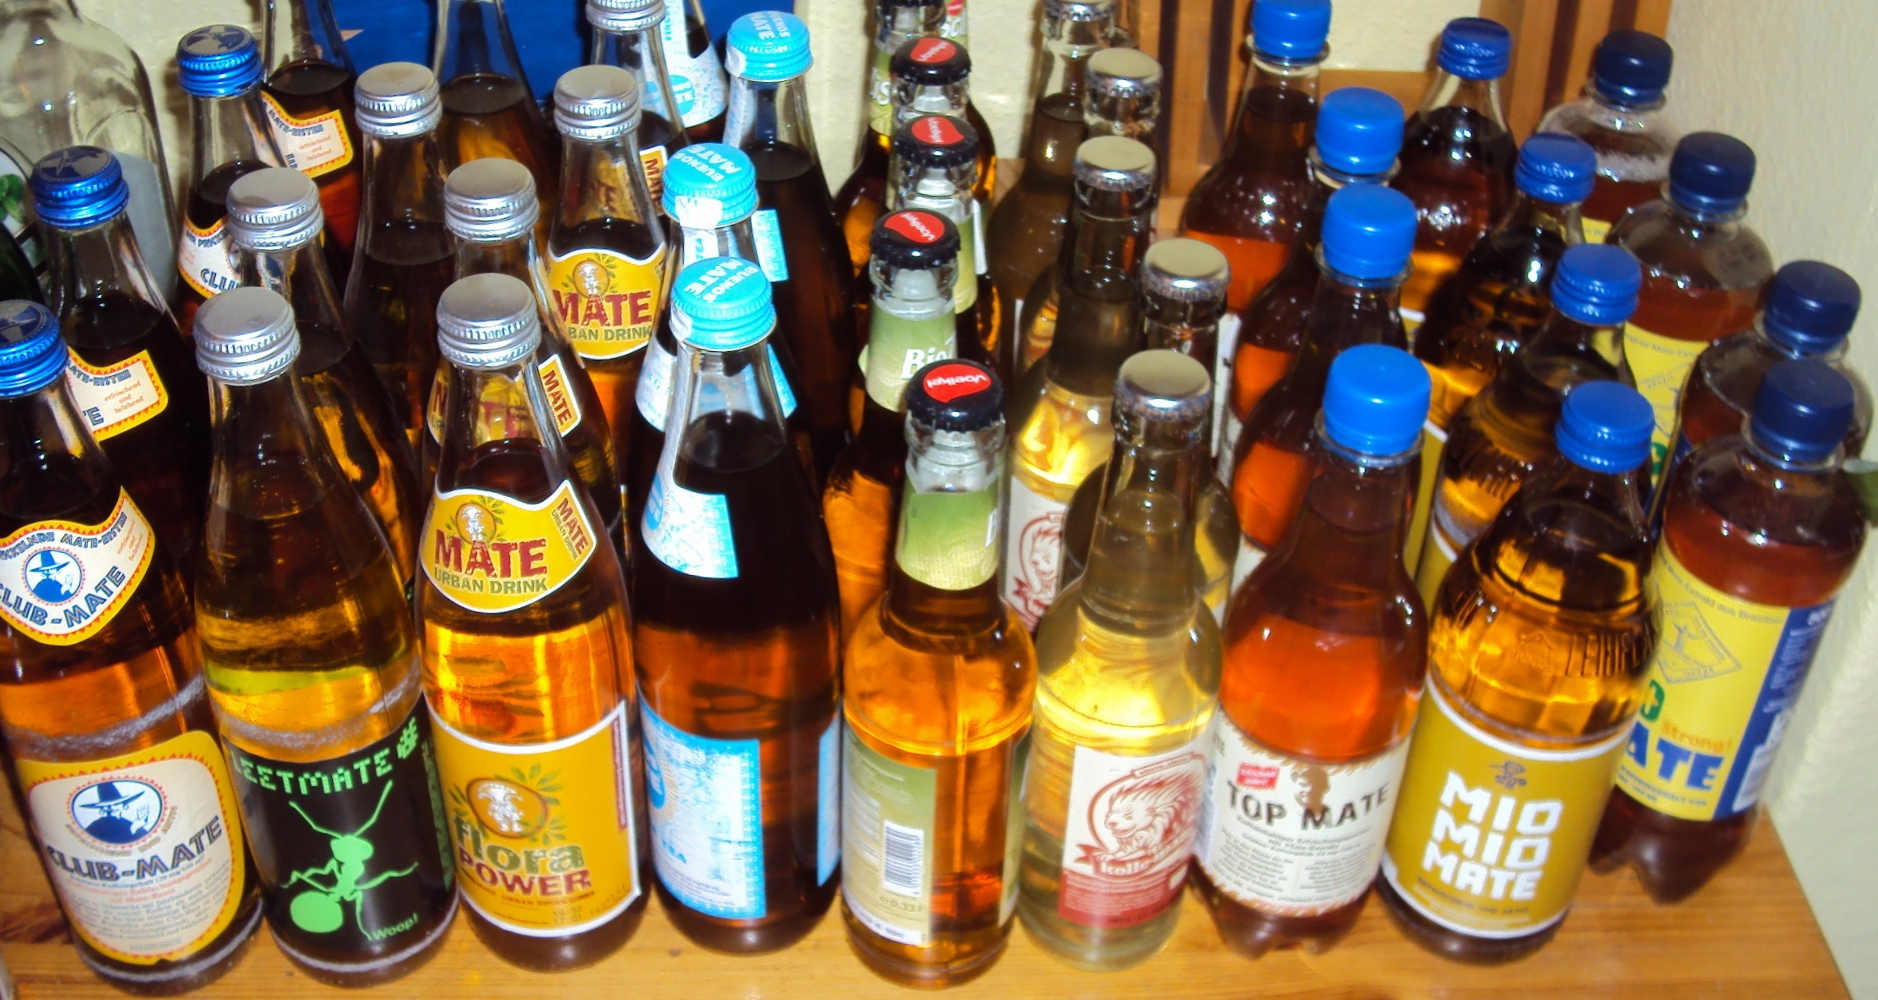
\includegraphics[width=0.8\textwidth]{./Fotos/Matesorten.JPG}
 \label{fig:flaschen}
\end{figure}

\subsection{Auswahl der Sorten}\label{sec:sorten-auswahl}
Das Ziel war es, eine möglichst große Auswahl an Mate--Sorten zu testen. Der Autorin war für sechs Sorten eine Bezugsquelle in Berlin bekannt. Auf diese hohe Zahl kommt es durch drei in der Nähe des Universitätsstandortes Adlershof im Kaufland geführte Mate--Sorten (Club, Buenos und MioMio) sowie den Bierhändler \href{http://www.ambrosetti.de/}{Ambrosetti} gegenüber vom ehemaligen Kindergarten der Autorin, welche FloraPower und 1337Mate führt. 

Beim Einkauf im Bioladen zusammen mit dem Vater der Autorin entdeckte diese zusätzlich noch BioZisch Mate und damit sah die Autorin eine genügend große Stichprobe für die Durchführung des Experiments gegeben und erstellte ein Facebookevent (siehe Abschnitt \ref{sec:stichprobe}).

Durch die \href{http://www.matekarte.de/}{matekarte} wurde die Autorin noch zusätzlich auf die Verfügbarkeit von TopMate aufmerksam und zwei der Gäste brachten auf eigene Initiative noch je eine weitere Sorte mit: Rio Mate und Kolle Mate. Die Verfügbarkeit letzterer ist besonders erwähnenswert, da Kolle--Mate in Berlin nicht im Verkauf erhältlich ist. Eine der Versuchspersonen hatte den Hersteller \textit{zickzack GmbH} angeschrieben und um die Zusendung einiger Flaschen gebeten. Diese erfolgte auch und zwar kostenfrei, lediglich mit der Bitte um eine Rückmeldung zum Geschmack ihrer Brause.\footnote{Dafür echt noch mal ein fettes Danke! Das war so cool von euch! :)\footnotemark}\footnotetext{hat unsere Neutralität in der Bewertung aber natürlich nicht beeinflusst}


\subsection{objektive Unterscheidungskriterien}\label{sec:objektives}
Der Geschmack der Mate ist natürlich ein wichtiger, aber eben auch völlig subjektiver, Faktor bei der Bewertung der Mate. Einige andere (einigermaßen) objektive Kriterien wurden aber im Umfeld dieser Studie zusammengetragen, um die Geschmacksbewertung zu ergänzen. Die vollständigen Daten hierzu sind Tabelle~\ref{tab:objektives} auf Seite~\pageref{tab:objektives} zu entnehmen.

\begin{description}
 \item[Preis] 
    Natürlich schwankt der Marktpreis für eine Sorte teilweise erheblich, es wurde jeweils der günstigste ermittelte Preis verwendet. Auf den Preis pro 0,5l umgerechnet schwankte dieser zwischen 0,55\euro (MioMio) und 1,49\euro (BioZisch) erheblich.

 \item[Verfügbarkeit] 
    Auf Berlin beschränkt, erfolgte eine grobe Abschätzung darüber, wie gut verfügbar die jeweilige Matesorte ist bzw. welche Bezugsquellen bekannt sind. Während der Marktführer ClubMate "`fast überall"' zu erhalten ist, ist für 1337Mate und FloraPower nur eine Bezugsquelle bekannt -- und für Kolle Mate gar keine in Berlin.

 \item[Flasche] 
    Die Flaschen unterscheiden sich in Material (Glas oder Plastik), in der Deckelfarbe (überwiegend blau) und auch in der Form. Hierfür ist jedoch keine objektive Rankingmöglichkeit gegeben.

 \item[Zuckergehalt] 
    Sofern dieser nicht explizit auf der Flasche angegeben war, wurde als Annäherung eine Schätzung über den Energiegehalt vorgenommen.
    Die Werte schwanken zwischen 4,2g/100ml (TopMate) und 5,8g/100ml (Kolle), welches Ende der Skala hier zu bevorzugen ist natürliche eine persönliche Entscheidung. 

 \item[Koffeingehalt] Da es sich um Getränke mit erhöhtem Koffenigehalt handelt, ist eine Angabe auf der Flasche gesetzlich vorgegeben. Die meisten Sorten haben einen Koffeingehalt von 20mg/100ml, leicht darunter liegt FloraPower (18mg/100ml), leicht darüber sind TopMate und 1337Mate (mit 22 bzw. 25mg/100ml) und -- mit deutlichem Abstand -- RioMate mit 32mg/100ml.
\end{description}



\subsection{Trinkerlebnis--Kriterien}
Zur Beschreibung des Trinkerlebnisses wurden die Verschpersonen gebeten die Sorten nach den folgenden Kriterien zu bewerten:
\begin{description}
 \item[Sprudeligkeit] 
    Das der Kohlensäure--Gehalt je nach Sorte deutlich zu schwanken scheint, war aus den Voruntersuchungen bekannt.

 \item[Geschmack] Die Beschreibung des Geschmackes beim Trinken war das Hauptaugenmerk der Untersuchung.

 \item[Skala Süß  $\leftrightarrow$ Herb] Neben einer Beschreibung des Geschmackes wurde um eine Einstufung gebeten, als wie süß dieser auf einer Skala eingeordnet würde.

 \item[Geruch] Nicht nur der Geschmack auch der Geruch sollte von den Probanden beschrieben werden.
\end{description}
  Zusätzlich gab es noch die Kategorie \textbf{Gesamturteil} und die Möglichkeit sonstige Bemerkungen abzugeben. Dies wurde unter anderem genutzt um Vermutungen zu der Sorte anzustellen.

\subsection{Vorurteile}
Einige Meinungen zu den Matesorten (vor Durchführung des Experiments) bei den Versuchspersonen waren:
\begin{enumerate}
 \item Top und Rio Mate können ja gar nicht schmecken, sind ja schließlich in Plastikflaschen.
 \item MioMio schmeckt voll eklig.
 \item FloraPower und 1337Mate sind am Besten.
 \item ClubMate hat viel zu viel Kohlensäure.
 \item ClubMate erkennt man auf jeden Fall leicht am Geschmack.
 \item Buenos schmeckt komisch.
\end{enumerate}


%+++++++++++++++++++++++++++++++++++++++++++++++++++++++++++++++++++++++++++++
\section{Versuchsdesign}
\subsection{Stichprobe}\label{sec:stichprobe}
Die Rekrutierung der Versuchspersonen (VP) erfolgte durch Erstellung eines "`Facebook--Event"'\footnote{\href{https://www.facebook.com/events/357170224387648/}{facebook.com/events/357170224387648/}} 
und Einladung aller als interessiert eingestuften und in Berlin lebenden "`Facebook--Freunde"' durch die Autorin. Dadurch kam es zu einer Teilnahme von 15 Personen (einschließlich der Autorin) an der Veranstaltung. Dies war eine deutlich höhere Anzahl als von der Autorin angenommen, weswegen die Wohnung der Autorin sehr voll wurde (siehe Abbildung~\ref{fig:wohnung} auf Seite~\pageref{fig:wohnung}). Weitere Angaben zu den Verschspersonen sind Tabelle~\ref{tab:VP} zu entnehmen.
%Hier sind Angaben zur Anzahl der Versuchspersonen, Geschlechterverhältnis, Muttersprache, Alter (\textit{M} und \textit{SD}), Studienfach und Belohnung zu machen.

\begin{table}[h!]
\centering
    \begin{tabular}{|>{\bfseries}l|p{6cm}|}
    \hline
    Anzahl der VP & $n=15$ \\
  \hline
    Geschlechterverhältnis & $6$ weiblich, $9$ männlich \\
  \hline
    Muttersprache & Alle VP haben (auch) Deutsch als Muttersprache. \\
  \hline
    Alter & . \\ %TODO: Alter
  \hline
    Studienfächer & 
	Mathematik: $6$,
	Informatik: $5$,
	Sonstige: $3$ (je 1 mal Chemie, Literaturwissenschaft und Technischer Umweltschutz) 
	 \\
  \hline
    Mate--Erfahrung & Alle VP waren zumindest mit Club Mate vertraut, keine der VP kannte vor dem Versuch alle getestete Mate--Sorten aus eigener Erfahrung.\\
  \hline
    \end{tabular}
\caption{Angaben zu den Versuchspersonen}
\label{tab:VP}
\end{table} 

\begin{figure}[ht]
 \centering
 \caption{Das mit VP überfüllte Wohnzimmer der Autorin}
 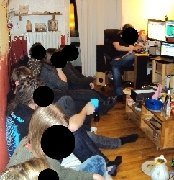
\includegraphics{./Fotos/Wohnung1.jpg}
 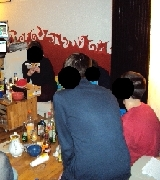
\includegraphics{./Fotos/Wohnung2.jpg}
 \label{fig:wohnung}
\end{figure}

\subsection{Material}
In dem Versuch verwendetes Material: 
\begin{itemize}
 \item vier bis sechs Flaschen Mate je getesteter Sorte  -- abhängig von beschaffender Person (vgl. Abschnitt~\ref{sec:sorten-auswahl}) und Flaschenvolumen                                                                                                                                                                                                                                                                                                                                                                                                   
 \item neun nummerierte Gläser zum anonymisierten Trinken (zu sehen in Abbildung~\ref{fig:glaeser} auf Seite~\pageref{fig:glaeser}) %TODO: anonymisiert verwendet man eig nur für Personen(daten), oder?
 \item einen Hut und Zettel mit den Matesorten zur Festlegung einer randomisierten Reihenfolge je Versuchsgruppe
 \item die Wohnung der Autorin, insbesondere mit:
  \begin{itemize}
    \item Küche für die jeweils aktive Versuchsgruppe
    \item Wohnzimmer zum Aufenthalt für die restlichen VP
    \item Flur zur Sammlung und Diskussion der Versuchsergebnisse
  \end{itemize}
 \item ein großes Plakat zum Notieren der Versuchsergebnisse (zu sehen in Abbildung~\ref{fig:plakat} auf Seite~\pageref{fig:plakat} im ausgefüllten Zustand)
\end{itemize}

\begin{figure}[hb]
 \centering
 \caption{Die nummerierten Gläser für das anonymisierte Trinken}
 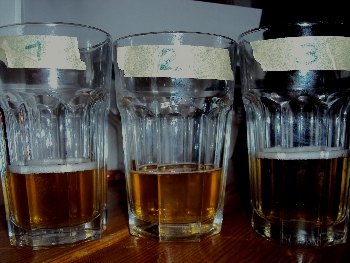
\includegraphics{./Fotos/Glaeser.jpg}
 \label{fig:glaeser}
\end{figure}

\begin{figure}[hb]
 \centering
 \caption{Die Versuchsergebnisse wurden zu einer vorläufigen Auswertung auf einem Plakat im Flur gesammelt}
 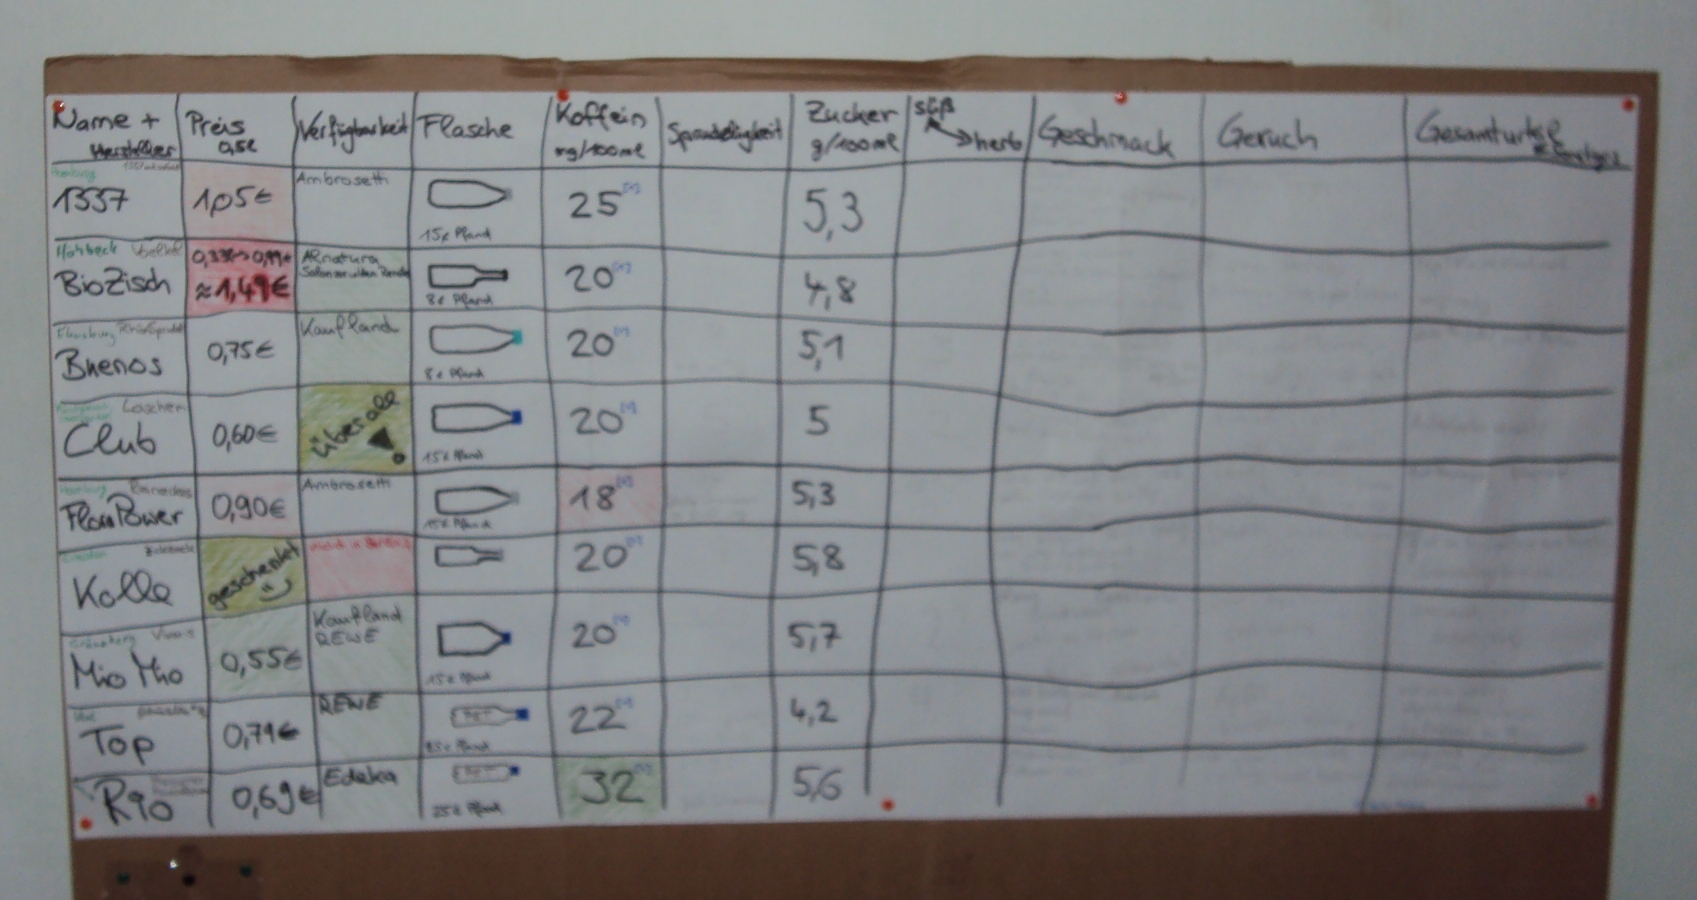
\includegraphics[width=\textwidth]{./Fotos/plakat.jpg}
 \label{fig:plakat}
\end{figure}



\subsection{Versuchsdurchführung} 
\begin{description}
 \item[Versuchsort:] die Wohnung der Autorin
 \item[chronologische Beschreibung des Versuchsablaufs:]~
  \begin{itemize}[label=-]
   \item Eintrudeln der VP
   \item Feststellen der Anzahl ($n=15$) und Aufteilen in fünf Gruppen mit je 3 VP
   \item Auslosen der Sorten--Reihenfolge für die erste Versuchsgruppe
   \item Eingießen der Mate--Sorten in die nummerierten Gläser gemäß ausgeloster Reiehenfolge
   \item Verkostung der Mate--Sorten und Ausfüllen der Tabelle durch die Versuchsgruppe
   \item Wiederholung der letzten 3 Schritte für jede Versuchsgruppe
  \end{itemize}
\end{description}




%+++++++++++++++++++++++++++++++++++++++++++++++++++++++++++++++++++++++++++++
\section{Ergebnisse}%TODO
\emph{Beinhaltet: Erklärung der verwendeten Maße, Deskriptive Darstellung ([1] nennen der Werte (z.B. \textit{M} und \textit{SD}) im Text; [2] Verweis auf Tabellen und Abbildungen zur Veranschaulichung), Statistische Darstellung (Varianzanalyse, t-Tests), gegebenenfalls weitere Auswertung. }

Die Rohdaten sind in Abschnitt \ref{sec:Rohdaten}


%+++++++++++++++++++++++++++++++++++++++++++++++++++++++++++++++++++++++++++++
\section{Diskussion der Ergebnisse}%TODO
\emph{Die Diskussion beinhaltet: Bezug zu den Hypothesen herstellen (bestätigt / nicht bestätigt), Interpretation der Ergebnisse, Auswirkungen dieser Befunde auf weitere Forschung, zugrundeliegende Theorien, auf die "`Realität"', konkrete/spezifische Idee(n) zu Folgeexperimenten (eine detailliertere genügt).}

%+++++++++++++++++++++++++++++++++++++++++++++++++++++++++++++++++++++++++++++
\section{Fazit}%TODO

%+++++++++++++++++++++++++++++++++++++++++++++++++++++++++++++++++++++++++++++


\begin{landscape}
\appendix 
\section{Rohdaten}\label{sec:Rohdaten}
\subsection{intrapersonelle Daten}\label{tab:objektives}
Wie in Abschnitt~\ref{sec:objektives} beschrieben, wurden einige "`objektive"' Daten zu den getestete Mate--Sorte zusammen getragen.

\begin{longtable}{|l||p{1.5cm}|R{2.3cm}|R{6cm}|p{2.3cm}|p{2.4cm}|}
  \hline
    Matesorte & Preis pro 0,5l & Verfügbarkeit &Flasche &Zuckergehalt in g/100ml &Koffeingehalt in mg/100ml\\
  \hline \hline
  \endhead 
    1337 & 1,05\euro & nur Ambrosetti & 0,5l Glasflasche mit silbernem Schraubverschluss--Deckel & 5,3  & 25 \\
  \hline
    BioZisch & 1,49\euro  & Alnatura, Salon zur wilden Renate & 0,33l Glasflasche   & 4,8  & 20 \\
  \hline
    Buenos & 0,75\euro  & Kaufland  & 0,5l Glasflasche mit hellblauem Schraubverschluss--Deckel  & 5,1 & 20\\
  \hline
    Club & 0,60\euro  & (fast) überall  & 0,5l Glasflasche mit dunkelblauem Schraubverschluss--Deckel  & 5  & 20 \\
  \hline
    Flora & 0,90\euro  & nur Ambrosetti  & 0,5l Glasflasche mit silbernem Schraubverschluss--Deckel  &  5,3  & 18 \\
  \hline
    Kolle & geschenkt  & nicht in Berlin  &  0,33l Glasflasche  & 5,8  & 20 \\
  \hline
    MioMio & 0,55\euro  & Kaufland, REWE  & 0,5l Glasflasche in spezieller Form (kleiner und bauchiger) mit dunkelblauem Schraubverschluss--Deckel  & 5,7  & 20 \\
  \hline
    Rio & 0,79\euro  & REWE  & PET--Flasche mit blauem Deckel & 5,6 & 32  \\
  \hline
    Top & 0,69\euro  & Edeka  & PET--Flasche mit blauem Deckel & 4,2 & 22   \\
  \hline
\end{longtable}



\subsection{Angaben der VP}
\begin{longtable}{|l|l||R{2cm}|R{2.2cm}|R{3.5cm}|R{4cm}|R{4cm}|} 
	\hline
	Sorte & Gr. & süß (1) $\leftrightarrow$ herb (5) & Sprudeligkeit, Schaum & Geruch & Geschmack & Gesamturteil/ sonstiges\\
	\hline\hline
  \endhead 
	\hline
	Mate Sorte & Gr. & süß(1) $\Leftrightarrow$ herb(5)  & Sprudeligkeit, Schaum & Geruch & Geschmack & Gesamturteil/ Sonstiges\\
	\hline\hline
  \endfirsthead
  \multicolumn{7}{c}{\textit{Fortsetzung auf der nächsten Seite}}
  \endfoot
  \endlastfoot

 \multirow{5}{*}{BioZisch}
 & 1 & weder süß noch herb & 3 (2) & 4 (3) & sauer, wenig matig & 1-2\\
\cline{2-7}
 & 2 & 5 & 3 & Eistee & säuerlich & Top! Großer Geschmacksakkord. Vermutung: 1337Mate\\
\cline{2-7}
 & 3 & 4 & 2 & zitronig, stark & herb-salzig, sojasaucenartig&voller, spezieller Geschmack\\
\cline{2-7}
 & 4 & 3 & 1,5 & Henna :( & nach Orange, nicht rund, Disharmonie im Geschmack & bäh\\
\cline{2-7}
 & 5 & $\pi\approx3,14$ & 2 keine Schaumkrone & grüner Tee, Eistee & leicht zitronig, Eistee, grüner Tee& Urteil: C, Vermutung: Buenos\\
\hline\hline\hline

 \multirow{5}{*}{Buenos}
 & 1 & 3 & (3 -) 4& 3, sehr schwacher Geruch & schlechter Nachgeschmack & 1-2\\
\cline{2-7}
 & 2 & 1 am Anfang, 3 im Abgang & 4 & schwach & süßlich, zitronig, teeig & großer Geschmacksakkord. Vermutung:Buenos\\
\cline{2-7}
 & 3 & 2,5 & 3,5 bierartig & süß+stark & fischig, nussig, rauchig & festes Mundgefühl, runde Perlen\\
\cline{2-7}
 & 4 & 3 & 2 & muffig & besser als der Geruch & nicht gut\\
\cline{2-7}
 & 5 & $e\approx 2,7$ & 3 & riecht nach Kotze & eklig & tiefer Farbton, ins Nussige gehend, Urteil: F, Vermutung: TopMate\\
\hline\hline\hline

\multirow{5}{*}{Club}
 & 1 & 1-2 & 4 & 2 & Club Mate typisch, karamellig &  Urteil:2\\
\cline{2-7}
 & 2 & 3 & 5& nach Mate! & neutral & Vermutung:Club \\
\cline{2-7}
 & 3 & 2,5 süß & 5& süßlich, karamellig & säuerlich (ein Hauch vom Zitrus), kräftig, leicht rauchig & Vermutung:Club\\
\cline{2-7}
 & 4 & 2 & 4,5& herb& "`normal"'& Vermutung: ClubMate; Aufstoßgefahr erhöht!\\
\cline{2-7}
 & 5 & 4 & 2,5 & intensiver Kräutergeruch, riecht wie sie schmeckt & klassisch & Vermutung:Club, Urteil:B\\
\hline\hline\hline


\multirow{5}{*}{Flora}
 & 1 & 3  & 2-3 & 4 & leicht sauer & Urteil:5(4), zweitleckerste Mate im Test\\
\cline{2-7}
 & 2 & 4 & 4& teeig& fast wie [Buenos], aber süßer & Vermutung:Flora\\
\cline{2-7}
 & 3 & 3& 3 fluffige Schaumkrone -- schenell weg& leicht rauchig, leicht zitronig& voller Geschmack, süffig& Urteil:lecker\\
\cline{2-7}
 & 4 & erst 2, dann 4& 2 & matig & intensiv, erst süß, dann herb & \\
\cline{2-7}
 & 5 & 2& 1,5& riecht süß, nicht aufdringlich & wie (Mate)saft & hat irgendwas von Apfel; Urteil: C+\\
\hline\hline\hline

\multirow{5}{*}{Kolle}
 & 1 & 1 & 2 (3) & 3 (4) & lasch & Urteil: 3 (2), passt gut zu Gin\\
\cline{2-7}
 & 2 & 3& 3,5 superschaumig& teeig& teeig, zitronig& Sommertagsbrause\\
\cline{2-7}
 & 3 & 1-2, sehr süß, fruchtig, aber nicht künstlich& 2& fruchtig& Apfel, leicht rauchig& \\
\cline{2-7}
 & 4 & 3 & 4 & citrus, sauer & erst süß-fruchtig, dann Grüntee, dann wieder süß & sehr gute Geschmackskomposition \\
\cline{2-7}
 & 5 & 2 & 2,5 & blumig, süß& Mate mit Blütensirup & klar, wenig Schaum, Urteil:B+\\
\hline\hline\hline

\multirow{5}{*}{Leet}
 & 1 & 3-4& 3& 5& & Urteil:5, leckerste Mate im Test\\
\cline{2-7}
 & 2 & 3 schaumbildend& 3& wie im Teeladen & matig & \\
\cline{2-7}
 & 3 & stark süße, aber keine voll Süße, leicht künstlich& 1& teeig, plasteartig& unvoll, wässerig & \\
\cline{2-7}
 & 4 & 1& 3& herb& nichtssagend süß, quietschig & nicht so gut \\
\cline{2-7}
 & 5 & 2,2 & 2& Kräuter, Eistee& eher wie Matetee, flüchtig& Bierfatamorgana, Urteil: B\\
\hline\hline\hline

\multirow{5}{*}{MioMio}
 & 1 & 2 & 4& schwacher Geruch, 3-4 & unerwartet & Urteil:1-2\\
\cline{2-7}
 & 2 & 2& 3& leicht, teeig, fast neutral & süßlich-snthetisch & anders süß als [RioMate]\\
\cline{2-7}
 & 3 & fruchtiger, süßer als [Club]& 4& süßlich, beerig& blumig, leicht herb& Vermutung:Flora\\
\cline{2-7}
 & 4 & 4& 3& nicht markant& nicht sehr intesiv, ein Hint von Waldmeister & interessant\\
\cline{2-7}
 & 5 & 4,5 & 2 & kaum wahrnehmbar, leicht nach Kräutern & 1. Schluck: Club Mate; 2.~Schluck: nee, irgendwas anderes, 3.~Schluck: bääh& Urteil:B$\rightarrow$ C $\rightarrow$ D\\
\hline\hline\hline

\multirow{5}{*}{Rio}
 & 1 & weder süß noch herb & 5 & 1 & Gummibärchen, künstlicher Erbeergeschmack & Urteil: 0\\
\cline{2-7}
 & 2 & 2 & 2 schaumbildend & fruchtig, zitronig & mild, weniger teeig & Einsteigermate, für Cocktails geeignet, unwachsig; Urteil: interessant \\
\cline{2-7}
 & 3 & Süße ist künstlich und zu schnell weg& 3 feste Schaumkrone& fruchtig& beerig, Gummibärchen, künstlicher Nachgeschmack, Apfelsaft?& Vermutung:Rio \\
\cline{2-7}
 & 4 & 1& 1& Hefe, Erdbeere, Hefeweizen& Erdbeersekt, schmeckt nicht wie Mate & gut als Getränk - aber nicht als Mate\\
\cline{2-7}
 & 5 & 2& 1 hochgradig instabile Schaumkrone& Erdbeersirup& fruchtig, aber unbestimmt& Sommermate; Vermutung:Rio; Urteil: C-\\
\hline\hline\hline

\multirow{5}{*}{Top}
 & 1 & gar nicht süß, aber auch nicht doll herb & 3& 2-3& fad, schwach& Urteil:2, innerhalb der Gruppe stark unterschiedlich bewertet\\
\cline{2-7}
 & 2 & 4& 4&  & teeig, wässerig& gepanschter Mist, Urteil: schlecht\\
\cline{2-7}
 & 3 & wie [Rio], aber nicht so extrem & sehr sprudelig im Mund & künstlich, zitronig, apfelig & anfangs ApfelGeschmack & Gesamt \\
\cline{2-7}
 & 4 & 4 & 2& Apfelschorle& erst citrus, dann sehr herb (wie grüner Tee)& lecker\\
\cline{2-7}
 & 5 & 3 & 1,5 & Sirup& Geschmack: vorhanden. flüssiges Kräterwasser & abgestandenes Wasser, Urteil: D\\
\hline
\end{longtable}


% \section{Abbildungen}
% \section{~}
\end{landscape}


\end{document}
